\chapter{Courses and Schedule}

\section{Courses}

\subsection{PME5018 - Projeto Integrado de Sistemas Mecânicos}

This course offers a great understanding of the project of a mechanical system. Not focusing only in the calculations and design of the product, this course presents a systemic and conceptual analysis of the project spiral. This course was of great importance for the design of ETMICAE since this project can later become a marketable product.

Grade: A

\subsection{PTC5721 - Controle Ótimo I}

This course presents the basic concepts for the Optimal Control Theory using Dynamic Programming and Variational calculus. Even with limited application in my current project objectives, this course offered greater understanding of the control theory. Heavily focused on a mathematical approach to the solution of the control problems. The tools and knowledge acquired through this course can be used in later implementations and developments of the exoskeleton control presented in this work.

Grade: C

\subsection{PMR5014 - Controle Não Linear Aplicado a Sistemas \\ Mecânicos e Mecatrônicos}

This course presents control techniques designed for non-linear systems, where the applications of classic control methods are not satisfactory. Differing from the Optimal Control course, this one offers a more practical and computational approach to the control problem. During the course, many control exercises were proposed to the students and solved through the use of MATLAB\textsuperscript{\textregistered}.  The exoskeleton presents some non-linearities such as viscous friction and gravitational forces. For this reason, the design of a non-linear controller can be favorable for a good control of the exoskeleton. 
%During the course, the design and analysis of a non-linear control method for an upper limb exoskeleton with a  one degree of freedom was made.

Grade: B

\subsection{PMR5004 - Fundamentos do Projeto de Sistemas \\ Mecânicos}

Focused on the basic and executive project steps of a mechanical system. Differing from the other mechanical project course, this one heavily focuses on mathematical tools for the selection and design of mechanical parts and machines. This course was of great importance for the design of ETMICAE and future developments on the mechanical structure of the exoskeleton since it offered a deeper understanding and mastery of mechanical design.

Grade: B

\subsection{PMR5005 - Biomecatrônica e Biorobótica}

This course offers a great overview of Biomechatronics and Biorobotics, presenting concepts and theories of the human motor control and human dynamics and how to develop robotic systems for assistance and rehabilitation. The information obtained through this course was of great importance to better understand the major breakthroughs and challenges to the exoskeleton and assistive technologies, better directioning this present work. At the end of this course, the first iteration of a system identification method for the upper limb was applied, which would later develop into the elbow angle estimation chapter present in this work.

Grade: A

\subsection{PMR5240 - Sensores, Atuadores e Problemas Inversos Bayesianos em Medicina}

This course offers an in-depth approach to technologies and sensors applied to medicine problems, such as ultrasound, image analysis and electrical impedance tomography. Even though the subject strays from the main focus of this work, it presented many different technologies and strategies that can be later applied to the control of an exoskeleton (e.g. using ultrasound to determine the muscle contraction and, consequently, a motion intention).

Grade: A

% Adicionado só para ter uma melhor formatação

\clearpage

\section{Schedule} 

\begin{figure}[thpb]
      \centering
      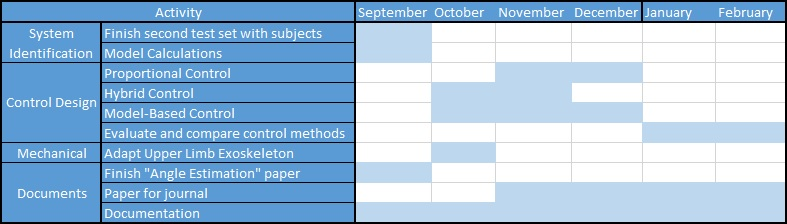
\includegraphics[width = \textwidth]{Images/Schedule.jpg}
      \caption{Schedule}
      \label{Schedule}
   \end{figure}